
\section{Aim and Organization of the Document.}

\subsection{Research questions.}

There are numerous research articles dealing with Wikipedia, notably
because this encyclopedia is used as a test base in information and
language processing systems\footnote{See, for instance, the researches conducted at University of Amsterdam,
\url{http://ilps.science.uva.nl/search/node/Wikipedia}.} and information retrieval tasks \citep{Burioletal06}.

This socio-technical project \citep{Bryantetal05,BenkerNissenbaum06},
where the tools used and the rules mediate and shape user activity
around open collaborative writing, can be seen as a community of practice
\citep{HaraShachafHew10}, or even as an aggregation of multiple communities
of practice (see, for instance, the analysis of the use of Wikipedia
by sport fans by \citealp{Ferriter09}). Regarding its functioning,
\citet{Okoli09,Park11,Okolietal12} may have proposed the most recent
review of the literature, which can be split into three main themes
(we add recent references to his): motivations to contribute \citep{Nov07},
and link between these motivation and the quality of the contribution
\citep{GlottSchmidtGhosh10b}; editorial process or internal organization
\citep{BestenDalle08,BrandesLerner08,Freardetal10,Kitturetal07a,Kitturetal07b,Ortega07}
and its impact on quality \citep{Viegasetal07,ViegasWattenbergMcKeon07,OkoliOh07,Stviliaetal08,CarilloOkoli11},
with a majority of article in Information System (IS), Computer Mediated
Communication and Computer Supported Cooperative Work; quality and
reliability of the production, with a more communication and library
science \citep{Denningetal05,Magnus06,Svoboda06,Gorman07,Waters07,Fallis08,Dede08,Fiedler08,Eijkman08,Rector08,SantanaWood09,WestWilliamson09,RoyalKapila09,Chen10}
and teaching orientation \citep{Callisetal09,Haigh11}, with more
critic studies before 2007, even if \citet{Giles05} is the first
publication which proposed a comparison of both Wikipedia and classical
encyclopedia, quite in favor of the first\footnote{For an example of the dialog between Librarian and Wikipedian, one
can look at the Wikipedia Loves Libraries manifestation, \url{http://en.Wikipedia.org/wiki/Wikipedia:Wikipedia_Loves_Libraries}.
For an overlook at the principal critics of Wikipedia, being pertinent
or not, see \citet{ONeil10}. }.

As we want to study the findings of all these articles, we need a
more general framework of understanding of the functioning of these
communities, before going deeper in their analysis. 

\subsection{A framework to analyze the project.}

\citet{CarilloOkoli11}'s framework (figure \ref{fig:Model-of-group},
page \pageref{fig:Model-of-group}) is rather extensive on the input
and process part, but less complete on the output part, as they only
focus on the declared quality of the articles by Wikipedia (''regular
article with no nomination, featured article nominees that were not
accepted, and featured articles''). 

\begin{figure}
\caption{\label{fig:Model-of-group}Model of group processes in open content
communities, from \citet{CarilloOkoli11}, figure 1 page 210.}

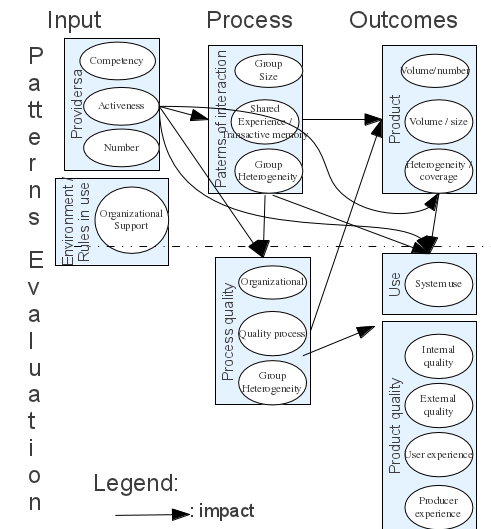
\includegraphics{Model_group_processes_open_communities_carillo_okoli}
\end{figure}

They did not explicitly take into account the retroactions, and did
not distinguish between the outcomes of the project and the specific
outcomes for the participants. One of the main differences between
these online projects (''communities'') and the other common good
productive communities is that the production outcomes (the pieces
of software, the Wikipedia articles) are available to all, when the
producers may have extra outcomes (and costs) to their involvement,
as we showed in \citet{JullienRoudautleSquin11}. 

For instance, \citet{CrowstonHowisonAnnabi06}, followed by \citet{LeeKimGupta09},
propose indicators to analyze the group production (they name ''system
creation''), and complete this model on two points. Relying on \citet{DeLoneMcLean92,DeLoneMcLean02,DeLoneMcLean03},
they proposed indicators to link the concrete outputs (here article,
in their case, open source software) to the user's satisfaction. In
their study, they also refer to \citet{Hackman87}, to show the importance,
as an output, of taking into account the producers (or contributors)
feedback, and the process of development to have a global view of
the outputs of such open online projects. They finally rely on \citet{Seddon97}
to extend Delone and McLean's model on the user side, with the concept
of ''perceived usefulness'', which echoes psycho-sociological studies
on the adoption of systems by users, such as Technology acceptance
model by \citet{Davis89} and its extensions \citep{Venkateshetal03}. 

Finally, Wikipedia is an example of a ``knowledge commons'' \citep{HessOstrom06b}.
These authors proposed a framework to understand the production of
such common, we present in figure \ref{fig:Institutional-Analysis-and},
page \pageref{fig:Institutional-Analysis-and}.

\begin{figure}
\caption{\label{fig:Institutional-Analysis-and}Institutional
Analysis and Development framework for knowledge commons \citep[p. 44]{OstromHess06}}
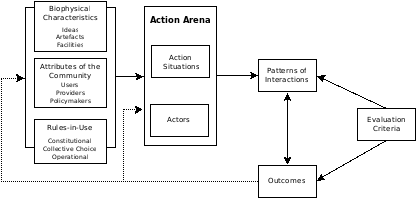
\includegraphics{Institutional_Analysis_and_Developement_framework_Hess-Ostrom}
\end{figure}

This leads us to a more global scheme (figure \ref{fig:Input,-process-and},
page \pageref{fig:Input,-process-and}), where inputs are the providers
as actors, the process the action arena (action situations) and mainly
the patterns of interaction, and the outputs, the outcomes, view from
different viewpoints, users, but also producers (providers in Hess
and Ostrom's terminology), and which can be seen as an extension of
the model proposed by \citet[p. 720]{ZhaoBishop11}. 

\begin{figure}
\caption{\label{fig:Input,-process-and}{Inputs,
process and outcomes of online open projects.}}
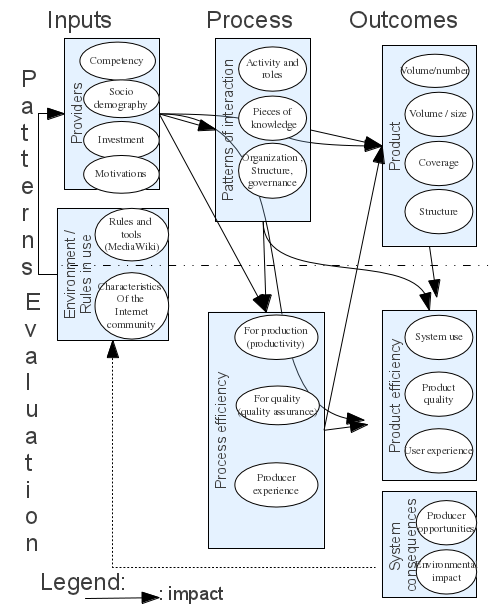
\includegraphics{New_model_of_group_processes_in_open_content_communities}
\end{figure}

Of course, as mentioned by the authors quoted, and what clearly appears
on Hess and Ostrom's framework, the outcomes influence the inputs.
The providers are given opportunities by their participation, leading
them to potentially involve more themselves in the project; the users
may also, by interacting with the system, become providers: for instance,
\citet{Lih04} shows that articles cited by the press see the number
of contributors increasing. We will come back to this point in the
conclusion of the article, but we argue that, before looking at how
this retro action loop works and impact the system, we have to understand
the system, which is the main goal of this work.

\subsection{The scientific production on Wikipedia.}

In concrete this means that a large part of the literature is out
of the scope of this article: neither the impact of the project on
the environment (the doted line in Figure \ref{fig:Input,-process-and}),
such as how it is used to comply professional tasks (by the students,
the researchers, the people in the industry), nor the analysis of
the propositions to improve the tools (using it on mobile, creating
a 3D Wikipedia), nor the use of Wikipedia as a database for information
retrieval test will be looked at here. This restriction does not provide
any restriction in terms of scientific scope (except for algorithm
research, data-mining, computational intelligence, semantic, information
retrieval), and we decided not to restrain our research to a particular
field as the topic is covered by various fields and as our goal was
to have an as extensive as possible view of the Wikipedia phenomenon. 
% * <nicolas.jullien@telecom-bretagne.eu> 2017-09-08T08:44:50.210Z:
% 
% From here, things have to be changed, according to what aer added
% 
% ^ <nicolas.jullien@telecom-bretagne.eu> 2017-09-08T08:45:44.621Z.
This is also the reason why we did not restrain to articles published
in journals, but added conference proceedings and books. However,
we restrain to papers published in English, French and Spanish as
we needed to understand the topics covered, and papers available before
February 2012.

We thus opted for a search strategy with high sensitivity \citep{DiestePadua07},
meaning that we searched with the keyword ''Wikipedia'' (or ''Wikip{\'{e}}dia)''
in the digital libraries (and not ''Wikipedia organization'', ''Wikipedia
evaluation'' or other terms which would have restraint the search),
in the title or keywords, but not in full text or in the summary as
we wanted that Wikipedia was specifically studied and not just an
example given in the text.

The original searches were conducted in December 2011 on Scorpus and WebofScience
databases. Bibliography for all the publications was stored in the
external bibliography system (CSV file and then Bibtex)\footnote{The query on Scopus was:

(TITLE(Wikipedia) OR TITLE(Wikip{\'{e}}dia) OR KEY(Wikipedia) OR KEY(Wikipédia))
AND (LIMIT-TO(DOCTYPE, ''cp'') OR LIMIT-TO(DOCTYPE,
''ar'')) AND (LIMIT-TO(LANGUAGE, ''English'')
OR LIMIT-TO(LANGUAGE, ''Spanish'') OR LIMIT-TO(LANGUAGE,
''French'')) AND (EXCLUDE(EXACTKEYWORD,
''Semantics'') OR EXCLUDE(EXACTKEYWORD,
''Information retrieval'') OR EXCLUDE(EXACTKEYWORD,
''Natural language processing systems'')
OR EXCLUDE(EXACTKEYWORD, ''Ontology'') OR
EXCLUDE(EXACTKEYWORD, ''Computational linguistics''))
AND (EXCLUDE(SUBJAREA, ''MATH'')) AND (EXCLUDE(EXACTKEYWORD,
''Artificial intelligence'') OR EXCLUDE(EXACTKEYWORD,
''Data mining''))}. We rejected introductions of panels, conferences, book reviews,
news flashes. We also deleted conference articles which were redundant
in the base, mostly because they had been presented in conferences
before been published in a journal, which let us with a bit less than
300 articles we read. Finally, we compared and completed the list
obtained looking at the list of the ''academic studies on Wikipedia''
maintained by the project itself\footnote{\url{en.wikipedia.org/wiki/Wikipedia:Wikipedia_in_academic_studies}}.

A first version were published in 2012. This version originates from this first version, and added references from there.

The rest of the article presents and discusses their findings, and
is organized accordingly to the framework proposed in figure \ref{fig:Input,-process-and}.